% Original reviewed schematic, 6 November 2026.
\begin{figure}[htbp]
\centering
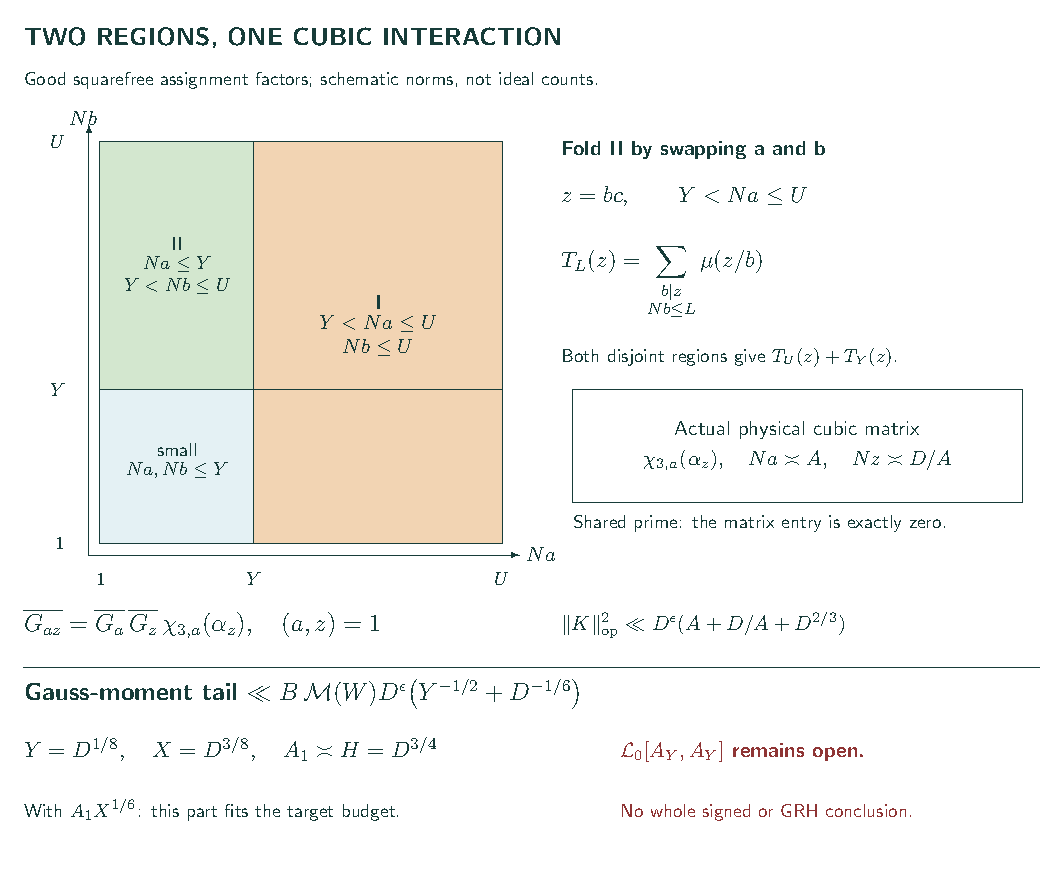
\includegraphics[width=\textwidth]{figures/gauss-tail-partition.pdf}
\caption{The two disjoint cutoff regions fold into the exact coefficient
$T_U+T_Y$, followed by the physical cubic matrix on coprime good squarefree
ideal factors. Norm axes are schematic, not ideal counts; a common prime
gives a raw zero. The displayed tail is the normalized Gauss moment,
not an energy or the raw numerator. The bound uses the explicitly cited
external cubic sieve. At $U\ge D^{1/8}$ the choice $Y=D^{1/8}$ fits the
stated pure critical error budget; if $Y=U$ the coefficient tail is zero.
The small-cutoff moment and the full kernel remain open.}
\label{gtl:partition}
\end{figure}
